\documentclass{article}

\usepackage{Sweave}
\begin{document}
\Sconcordance{concordance:05_results.tex:05_results.Rnw:%
1 2 1 1 0 15 1}



\section{Results}
Once we figured out which variable selection methods we wanted to use and how we wanted to use them, we were then able to implement them using a Shiny R App. A screenshot of the Shiny R app below shows exactly the options that a user has when running the web application:\\

\begin{figure}[!htb]
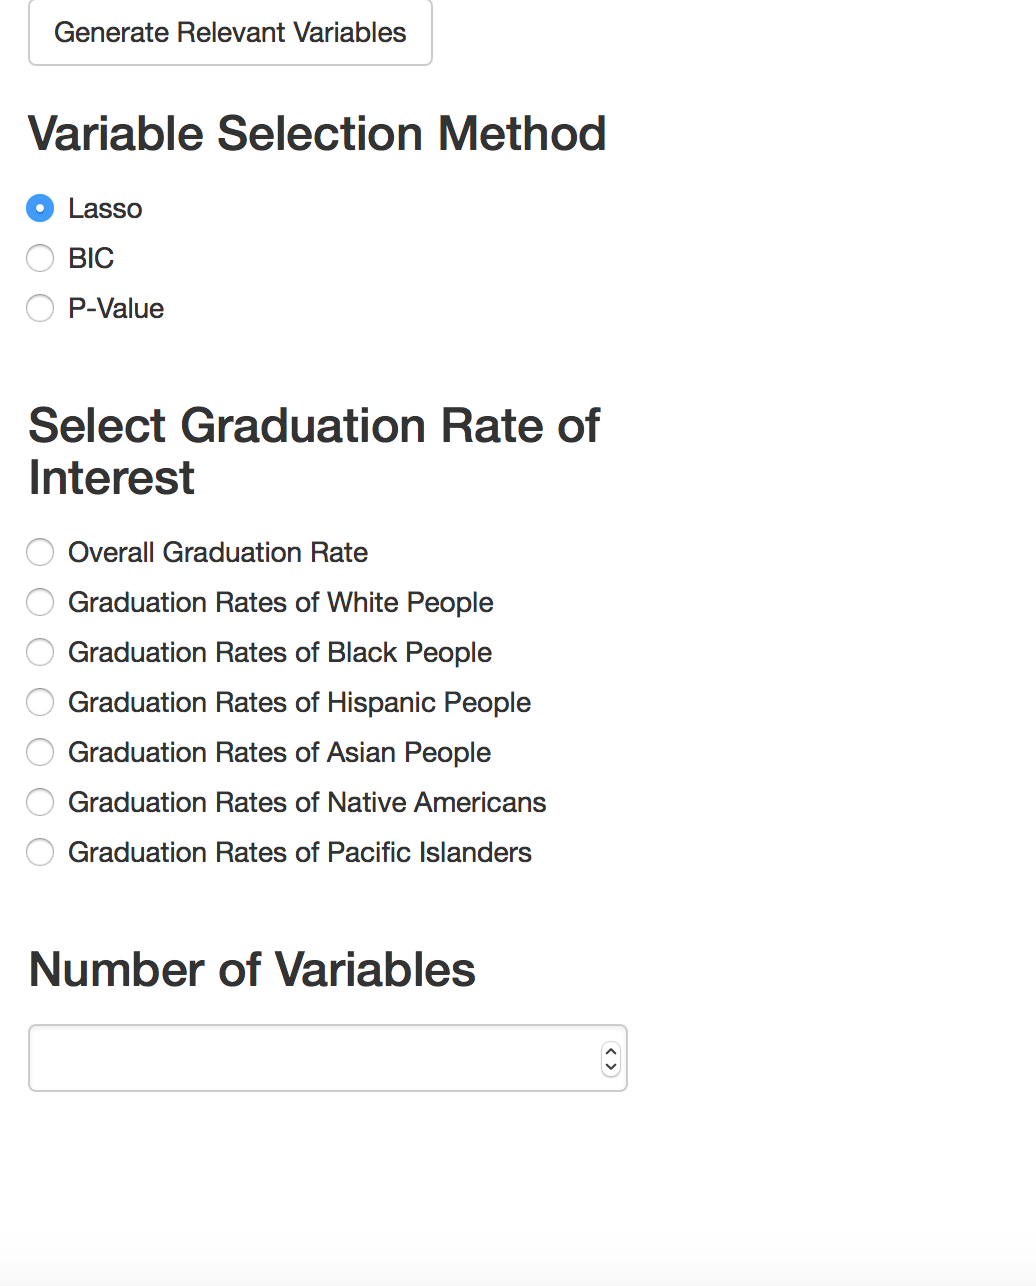
\includegraphics{../../images/screenshot.png}
\end{figure}


The Shiny R App will then output the specified number of relevant variables for the specified graduation rate. For instance, lets say we were interested in finding the 5 most relevant explanatory variables for the overall graduation rate. Then, we could get 3 sets of 5 explanatory variables (one set for each variable selection method). It turns out that the only explanatory variable that appears in all 3 variable selection methods is the SAT average variable, which has a strong positive effect on graduation rates. This makes sense because intuitively, SAT scores have a strong correlation with high academic performance, which is essential to graduating. 
\end{document}


